\documentclass[../sparc.tex]{subfiles}
\graphicspath{{\subfix{../images/}}}
\begin{document}

%%%%%%%%%%%%%%%%%%%%%%%%%%%%%%%%%%%%%%%%%%%%%%%%%%%%%%%%%%%%%%%%%%%%%%%%%%%%%%%%
\section{ЖК-дисплей}

Для вывода информации мы будем использовать \emph{жидкокристаллический дисплей}
(ЖК-дисплей), подключаемый к Arduino.  Принцип работы данных дисплеев аналогичен
обычным ЖК-дисплеям, которые выводят информацию на вашем компьютере.  Более
конкретно мы будем использовать \emph{текстовый} ЖК-дисплей, который
предназначен для вывода тестовых символов.

На текстовых ЖК-дисплеях, экран поделён на клетки, внутри каждой из которых
можно отрисовать один символ (букву, знак препинания, цифру, или просто
какую-либо картинку.)  Между клетками обычно находится расстояние в один
пиксель.  Подобные дисплеи плохо подходят для отрисовки произвольных
изображений, тем не менее, некоторый простор для творчества у нас имеется.

Несмотря на свойства дисплея, которые на первый взгляд кажутся слишком
ограничивающими для наших задач, используя наше мастерство и творческий подход,
мы можем добиться достаточно интересных результатов в плане разработки игр.

\subsection{Подключение дисплея}

Для упрощения нашей работы мы будем использовать ЖК-дисплей с интерфейсом
передачи данных, который называется ``I2C'' (читается ``ай-ту-си''.)  Не
вдаваясь в подробности можно сказать, что данный вариант подключения требует
всего 4 провода: питание, земля и две линии передачи данных.

Сам модуль I2C часто уже припаян к дисплею, но может идти и отдельно.  В случае
отдельного модуля, подключение выглядит, как на рис. \ref{fig:lcd-00}.

\begin{figure}[ht]
  \centering
  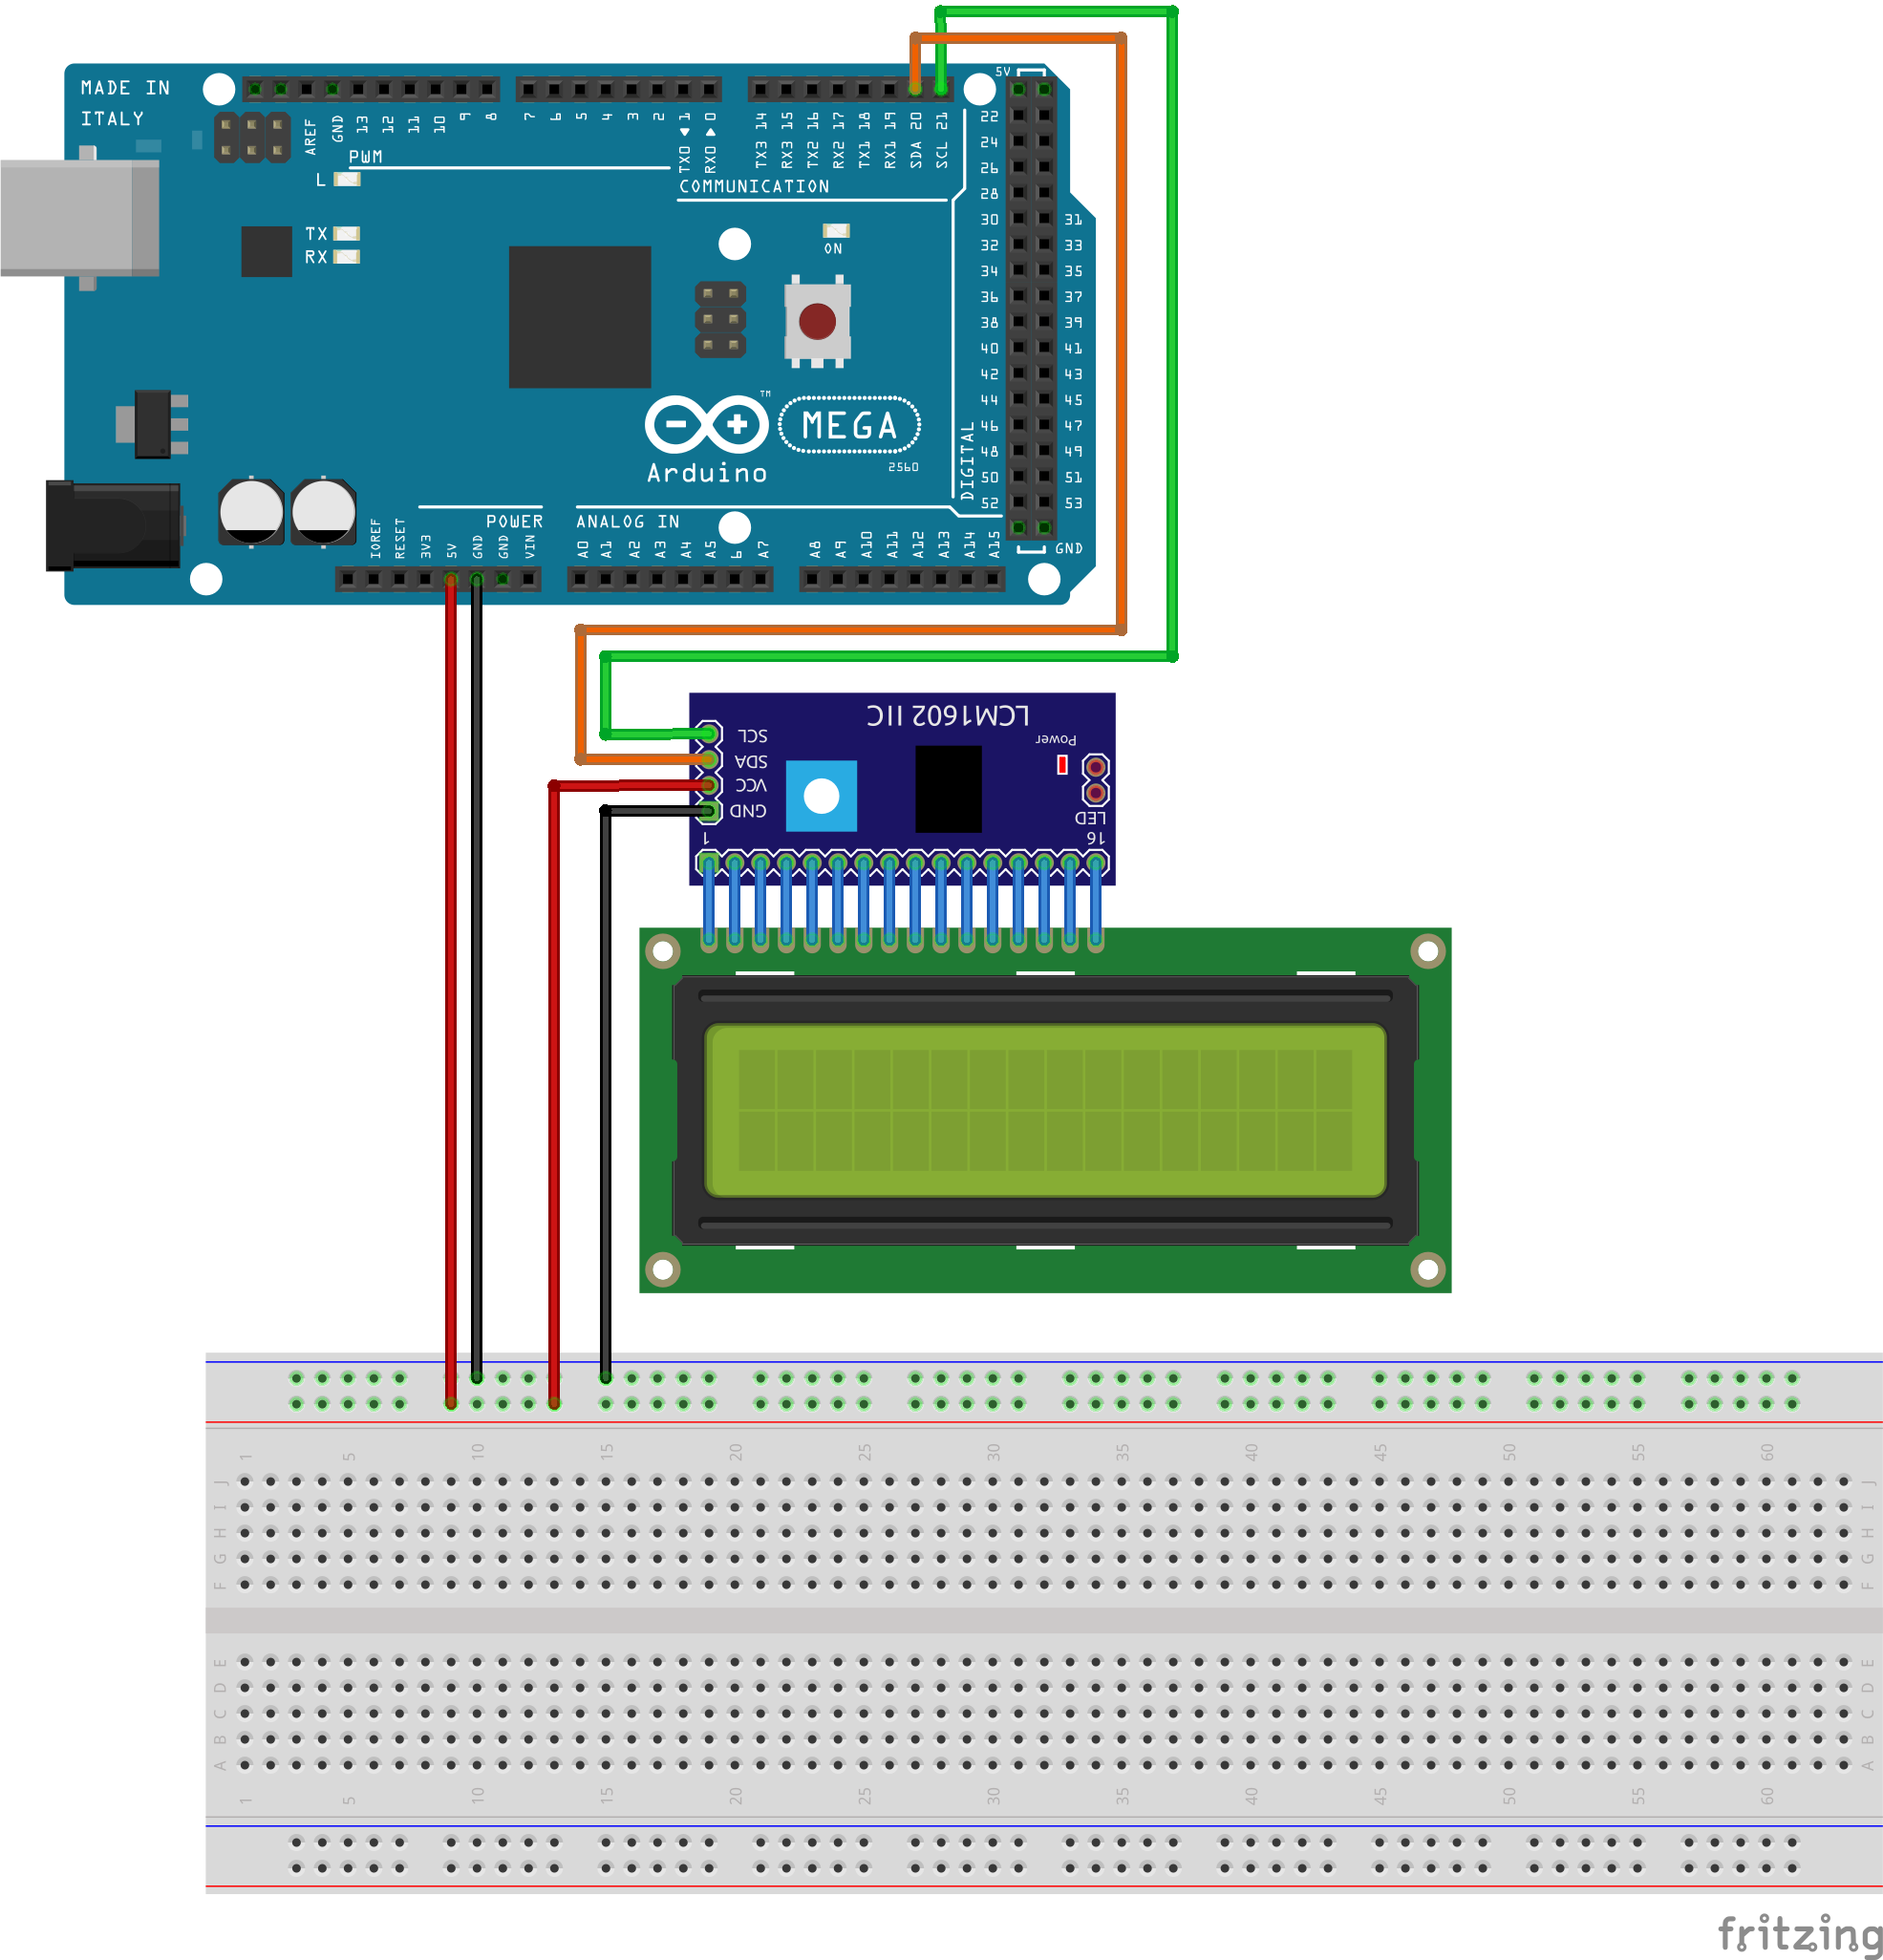
\includegraphics[width=12cm]{schematics/lcd-00}
  \caption{Схема подключения ЖК-дисплея 16x2 по интерфейсу I2C к Arduino Mega
    2560.}
  \label{fig:lcd-00}
\end{figure}

\subsection{Вывод текста}

Согласно традиции, первая программа, которую мы выведем -- это ``Привет, Мир!''.
Однако поскольку вывода русского текста на большинстве дисплеев организован
сложнее, нежели чем латинницы, то мы будем выводить ``Hello, World!''.

Для этого нам необходимо во-первых установить библиотеку для работы с дисплеем;
во-вторых настроить дисплей на нужный режим работы и только после этого мы
сможем вывести текст.

Начнём со скачивания библиотеки.  Проще всего это сделать через менеджер
библиотек, доступный из меню ``Инструменты'' (``Tools'').  Существуют несколько
библиотек, которые могут обеспечить работу ЖК-дисплея по протокола I2C.  Мы
можем взять библиотеку ``Liquid Crystal I2C'' версии 1.1.1 под авторством Марко
Шварца (Marco Schwartz).

Установив библиотеку, мы сможем использовать её функционал.

Первым делом в коде нам необходимо подключить библиотеку
\texttt{LiquidCrystal\_I2C.h} -- это делается через специальную команду
\texttt{\#include}.

\begin{minted}{cpp}
#include <LiquidCrystal_I2C.h>
\end{minted}

В глобальной области кода (до функции \texttt{setup} и \texttt{loop}) необходимо
создать специальную переменную, через которую мы будем работать с дисплеем.  Эта
переменная отличается от того, что мы видели раннее -- в данной переменной
хранится не число, а ссылка более сложный \emph{объект}, который располагается
где-то в памяти при работе программы внутри микроконтроллера.

\begin{minted}{cpp}
LiquidCrystal_I2C lcd(0x27,  16, 2);
\end{minted}

Далее в функции \texttt{setup} необходимо выполнить настройку дисплея.

\begin{minted}{cpp}
lcd.init();
lcd.backlight();
\end{minted}

После этого уже в функции \texttt{loop} мы можем вывести текст.  Вывод текста
как правило делается в два этапа: во-первых, необходимо установить место, в
которое будет ``впечатан'' текст.  Для этого существует специальная функция
\texttt{setCursor}.

\begin{minted}{cpp}
lcd.setCursor(0, 0);
\end{minted}

После этого наконец-то мы можем вывести текст.

\begin{minted}{cpp}
lcd.print("Hello, World!");
\end{minted}

Полностью код будет выглядеть примерно так, как показано ниже.

\begin{minted}{cpp}
#include <LiquidCrystal_I2C.h>

LiquidCrystal_I2C lcd(0x27,  16, 2);

void setup() {
  lcd.init();
  lcd.backlight();
}

void loop() {
  lcd.setCursor(0, 0);
  lcd.print("Hello, World!");
}
\end{minted}

\end{document}
